\documentclass[10pt]{article}
\usepackage[margin=0.75in]{geometry}
\usepackage{booktabs}
\usepackage{graphicx}
\usepackage{microtype}
\title{Persistent Update-Only Evaluation: Spine versus Trace-Aware GraSU}
\author{}
\date{July 31, 2026}
\begin{document}
\maketitle

We separate pure accelerator update throughput from the one-time CPU work that
makes a trace executable. No SSSP, PageRank, CC, convergence loop, or ReGraph
compute stage runs in either device-only measurement. The input is the full
directed AskUbuntu materialization (515,281 vertices and 390,847 initial
edges); every point contains ten persistent batches. All per-batch and final
graph-state checks pass.

\begin{figure}[h]
  \centering
  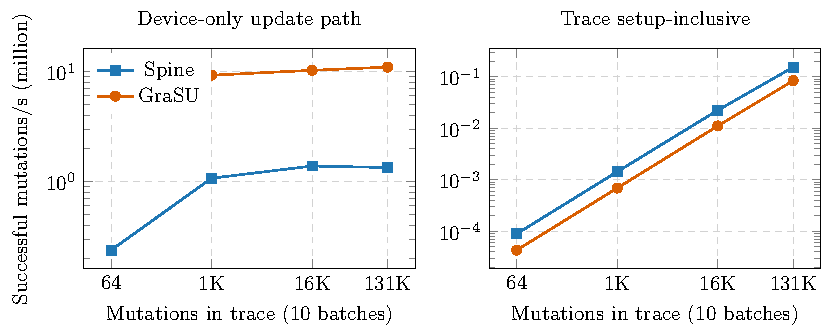
\includegraphics[width=\linewidth]{../figures/persistent_update_only_20260731.pdf}
  \caption{Successful insertion throughput. Left: pure structure-update device
  time. Right: measured CPU preprocessing plus simulated device time, with a
  shared parameterized 12 GB/s H2D and 10 $\mu$s launch/sync cost per batch.
  GraSU uses its official future-aware update-density reorder and reserves PMA
  slots once for the complete trace; Spine sees and sorts each arriving batch.}
\end{figure}

\begin{table}[h]
\centering
\begin{tabular}{rrrrr}
\toprule
Mutations & Spine device & GraSU device & Device speedup & Setup-incl. speedup \\
 & Mupd/s & Mupd/s & Spine/GraSU & Spine/GraSU \\
\midrule
64      & 0.238 & 5.327  & 0.045$\times$ & 2.076$\times$ \\
1,024   & 1.074 & 9.267  & 0.116$\times$ & 2.078$\times$ \\
16,384  & 1.385 & 10.278 & 0.135$\times$ & 2.017$\times$ \\
131,072 & 1.342 & 10.982 & 0.122$\times$ & 1.830$\times$ \\
\bottomrule
\end{tabular}
\end{table}

The PMA device path is 7.4--22.4$\times$ faster. The setup-inclusive ranking
reverses because GraSU's reorder and reserved-PMA construction costs about
1.47--1.54 s, compared with about 0.71--0.75 s for Spine preload and per-batch
sorting. This does not claim that Spine has a faster PMA update kernel. It shows
that GraSU's offline cost must be amortized over a sufficiently long known
trace. A future-unknown, online-rebalancing GraSU is a separate experiment.

\end{document}
